\documentclass[letter,11pt]{beamer}

%spell related
\usepackage[spanish,es-nodecimaldot]{babel}
\usepackage[utf8]{inputenc}

%fonts related
\usepackage{helvet}
\renewcommand{\familydefault}{\sfdefault}
\usepackage{textcomp}

%graphics related
\usepackage{adjustbox}
\usepackage{graphicx}
\usepackage{pstricks}

\usepackage{graphicx}
\usepackage{array}

\usetheme{Pittsburgh}
\setbeamerfont{frametitle}{size=\normalsize}

\title{\textbf{LABORATORIO DE FÍSICA BÁSICA I - TOMA DE DATOS}}
\subtitle{\textbf{Calibrador \emph{Vernier} - Tornillo micrométrico}}
\author{\small{Caballero Burgoa, Carlos Eduardo}}
\date{\tiny{Octubre 2020}}

\begin{document}

\begin{frame}
\titlepage
\end{frame}

\section{Calibrador \emph{Vernier}}

\subsection{Diámetro del circulo}
\begin{frame}
\frametitle{Diámetro del circulo}
\vspace*{0.8cm}
\begin{figure}
\centering
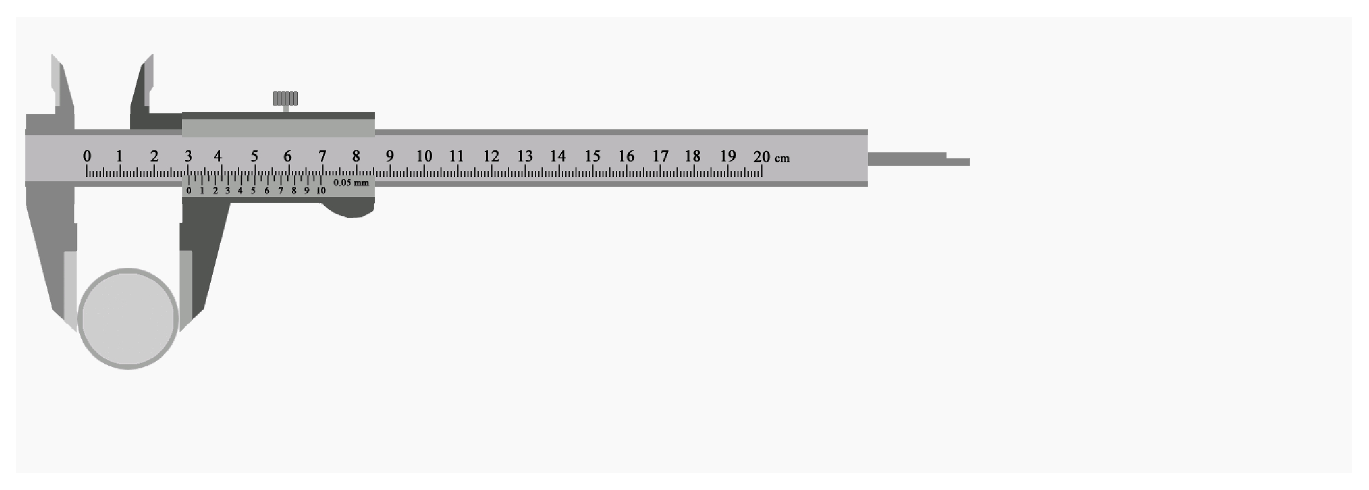
\includegraphics[width=1.0\textwidth]{resources/1_5.1.1.eps}
\end{figure}
\vspace*{0.4cm}
\scriptsize
\begin{tabular}{|c|>{\centering}m{1.8cm}<{\centering}|}
\hline
$X_{rep}$ &  $30.35$ \tabularnewline \hline
      $P$ &   $0.05$ \tabularnewline \hline
      $u$ &     $mm$ \tabularnewline \hline
$E_x(\%)$ &   $0.16$ \tabularnewline \hline
\end{tabular}
\quad
\begin{tabular}{|c|>{\centering}m{5.7cm}<{\centering}|}
\hline
\multicolumn{2}{|c|}{\textbf{Resultado de la medición}} \\ \hline
$D$ & $( 30.35\pm0.05)[mm], 0.16\%$ \tabularnewline \hline
\end{tabular}
\end{frame}

\subsection{Diámetro de la cabeza del perno}
\begin{frame}
\frametitle{Diámetro de la cabeza del perno}
\vspace*{0.8cm}
\begin{figure}
\centering
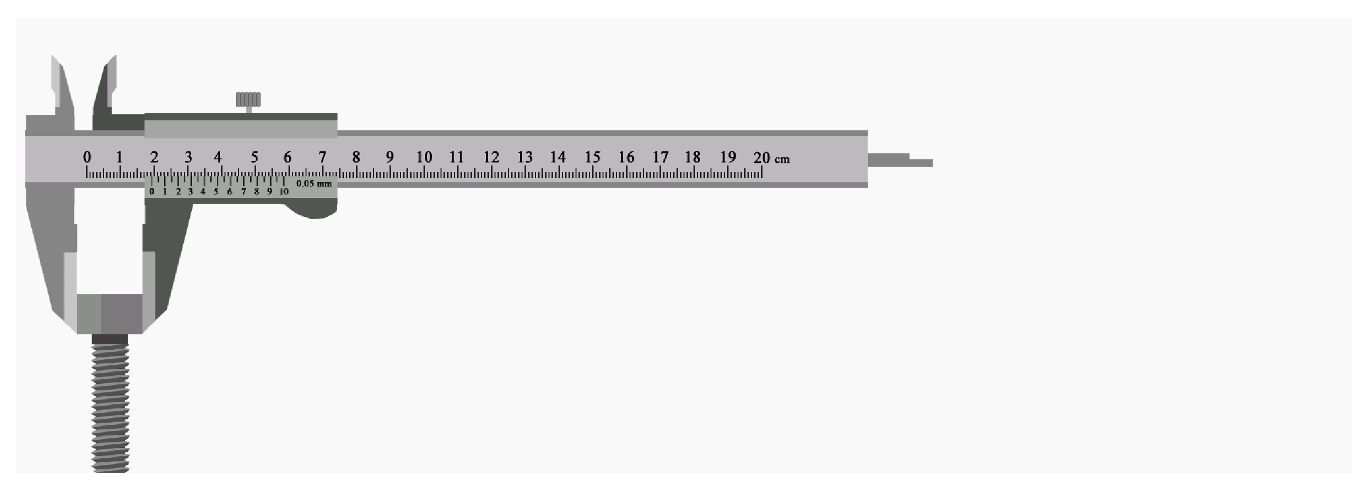
\includegraphics[width=1.0\textwidth]{resources/1_5.1.2.eps}
\end{figure}
\vspace*{0.4cm}
\scriptsize
\begin{tabular}{|c|>{\centering}m{1.8cm}<{\centering}|}
\hline
$X_{rep}$ &  $19.30$ \tabularnewline \hline
      $P$ &   $0.05$ \tabularnewline \hline
      $u$ &     $mm$ \tabularnewline \hline
$E_x(\%)$ &   $0.26$ \tabularnewline \hline
\end{tabular}
\quad
\begin{tabular}{|c|>{\centering}m{5.7cm}<{\centering}|}
\hline
\multicolumn{2}{|c|}{\textbf{Resultado de la medición}} \\ \hline
$D$ & $( 19.30\pm0.05)[mm], 0.26\%$ \tabularnewline \hline
\end{tabular}
\end{frame}

\subsection{Diámetro del cuerpo del perno}
\begin{frame}
\frametitle{Diámetro del cuerpo del perno}
\vspace*{0.8cm}
\begin{figure}
\centering
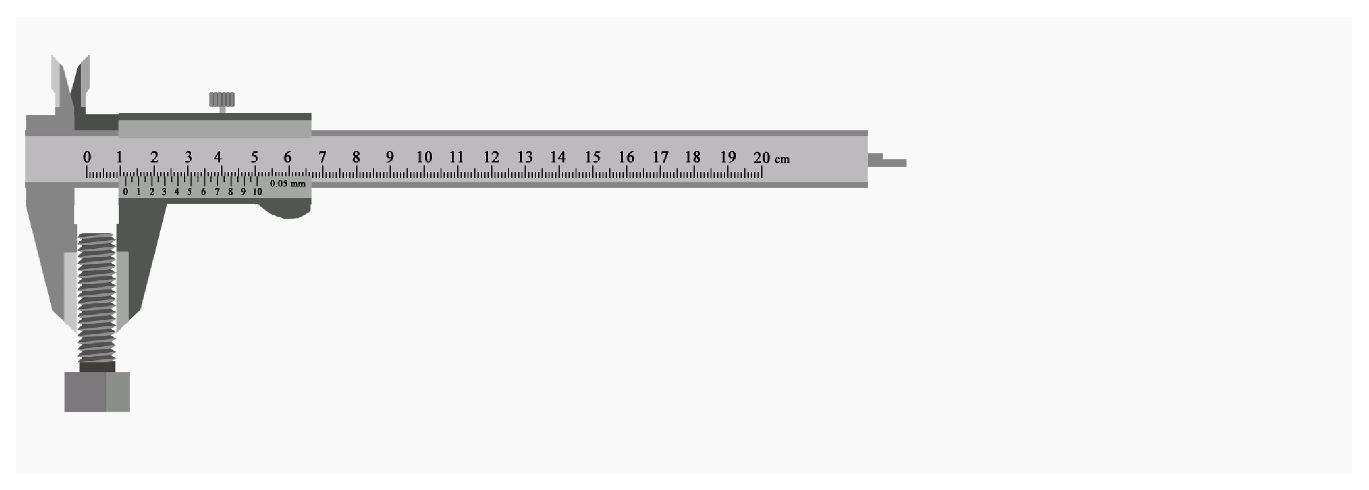
\includegraphics[width=1.0\textwidth]{resources/1_5.1.3.eps}
\end{figure}
\vspace*{0.4cm}
\scriptsize
\begin{tabular}{|c|>{\centering}m{1.8cm}<{\centering}|}
\hline
$X_{rep}$ &  $11.55$ \tabularnewline \hline
      $P$ &   $0.05$ \tabularnewline \hline
      $u$ &     $mm$ \tabularnewline \hline
$E_x(\%)$ &   $0.43$ \tabularnewline \hline
\end{tabular}
\quad
\begin{tabular}{|c|>{\centering}m{5.7cm}<{\centering}|}
\hline
\multicolumn{2}{|c|}{\textbf{Resultado de la medición}} \\ \hline
$D$ & $( 11.55\pm0.05)[mm], 0.43\%$ \tabularnewline \hline
\end{tabular}
\end{frame}

\subsection{Longitud de la cabeza del perno}
\begin{frame}
\frametitle{Longitud de la cabeza del perno}
\vspace*{0.8cm}
\begin{figure}
\centering
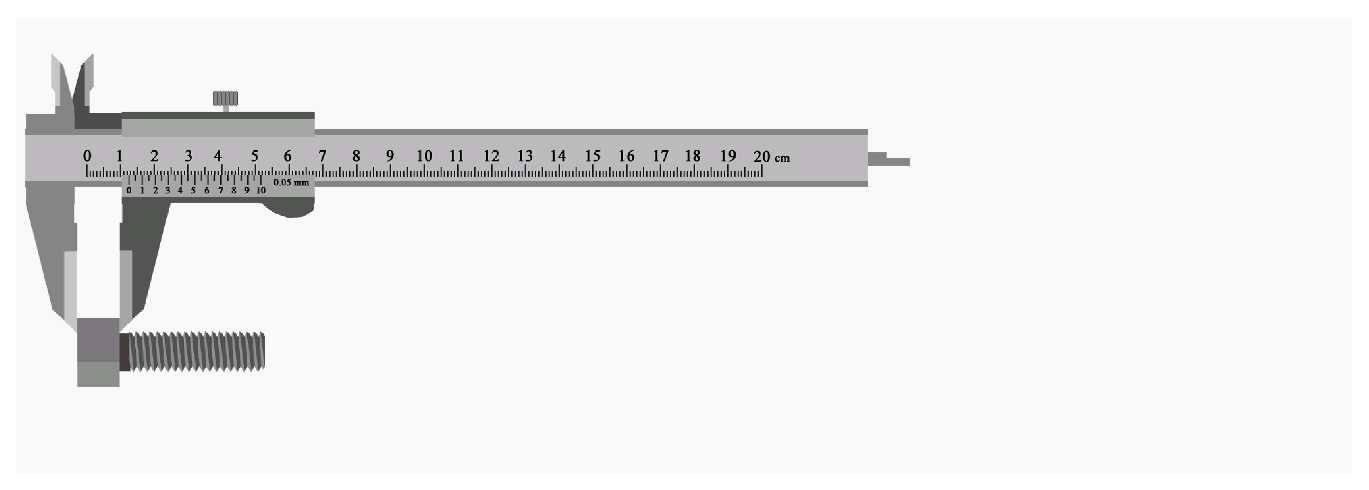
\includegraphics[width=1.0\textwidth]{resources/1_5.1.4.eps}
\end{figure}
\vspace*{0.4cm}
\scriptsize
\begin{tabular}{|c|>{\centering}m{1.8cm}<{\centering}|}
\hline
$X_{rep}$ &  $12.55$ \tabularnewline \hline
      $P$ &   $0.05$ \tabularnewline \hline
      $u$ &     $mm$ \tabularnewline \hline
$E_x(\%)$ &   $0.40$ \tabularnewline \hline
\end{tabular}
\quad
\begin{tabular}{|c|>{\centering}m{5.7cm}<{\centering}|}
\hline
\multicolumn{2}{|c|}{\textbf{Resultado de la medición}} \\ \hline
$L$ & $( 12.55\pm0.05)[mm], 0.40\%$ \tabularnewline \hline
\end{tabular}
\end{frame}

\subsection{Longitud del cuerpo del perno}
\begin{frame}
\frametitle{Longitud del cuerpo del perno}
\vspace*{0.8cm}
\begin{figure}
\centering
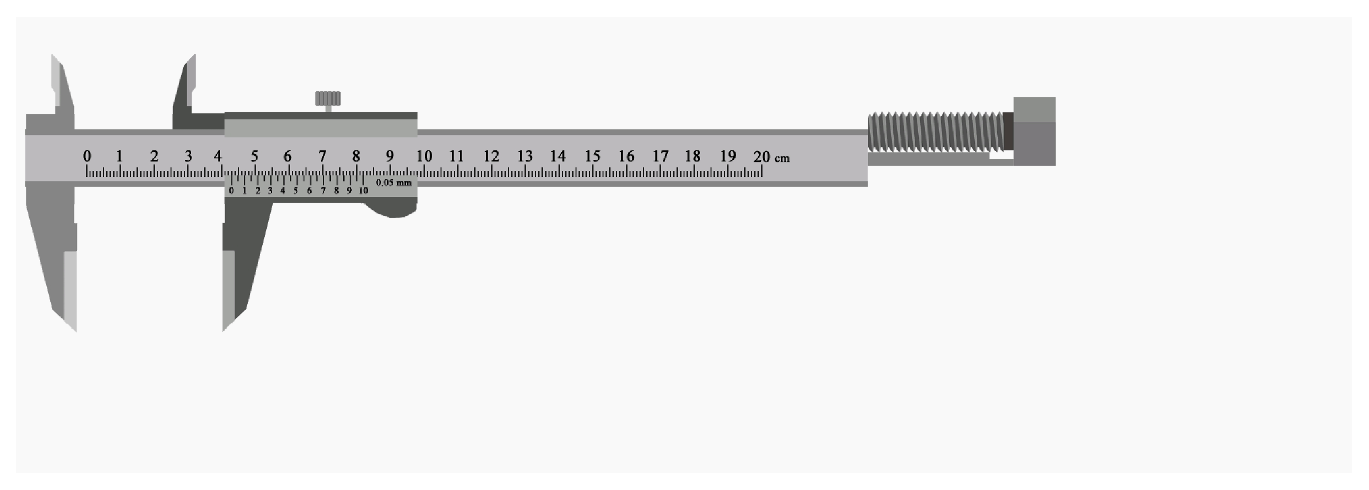
\includegraphics[width=1.0\textwidth]{resources/1_5.1.5.eps}
\end{figure}
\vspace*{0.4cm}
\scriptsize
\begin{tabular}{|c|>{\centering}m{1.8cm}<{\centering}|}
\hline
$X_{rep}$ &  $43.00$ \tabularnewline \hline
      $P$ &   $0.05$ \tabularnewline \hline
      $u$ &     $mm$ \tabularnewline \hline
$E_x(\%)$ &   $0.12$ \tabularnewline \hline
\end{tabular}
\quad
\begin{tabular}{|c|>{\centering}m{5.7cm}<{\centering}|}
\hline
\multicolumn{2}{|c|}{\textbf{Resultado de la medición}} \\ \hline
$L$ & $( 43.00\pm0.05)[mm], 0.12\%$ \tabularnewline \hline
\end{tabular}
\end{frame}

\subsection{Longitud total del perno}
\begin{frame}
\frametitle{Longitud total del perno}
\vspace*{0.8cm}
\begin{figure}
\centering
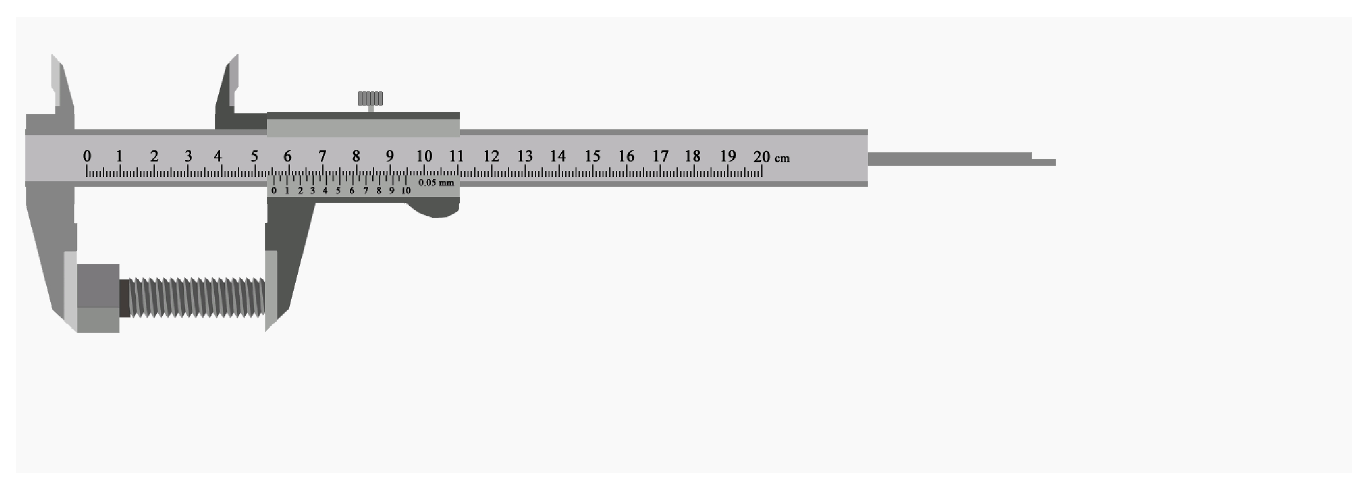
\includegraphics[width=1.0\textwidth]{resources/1_5.1.6.eps}
\end{figure}
\vspace*{0.4cm}
\scriptsize
\begin{tabular}{|c|>{\centering}m{1.8cm}<{\centering}|}
\hline
$X_{rep}$ &  $55.55$ \tabularnewline \hline
      $P$ &   $0.05$ \tabularnewline \hline
      $u$ &     $mm$ \tabularnewline \hline
$E_x(\%)$ &   $0.09$ \tabularnewline \hline
\end{tabular}
\quad
\begin{tabular}{|c|>{\centering}m{5.7cm}<{\centering}|}
\hline
\multicolumn{2}{|c|}{\textbf{Resultado de la medición}} \\ \hline
$L$ & $( 55.55\pm0.05)[mm], 0.09\%$ \tabularnewline \hline
\end{tabular}
\end{frame}

\subsection{Diámetro de la cabeza del tornillo}
\begin{frame}
\frametitle{Diámetro de la cabeza del tornillo}
\vspace*{0.8cm}
\begin{figure}
\centering
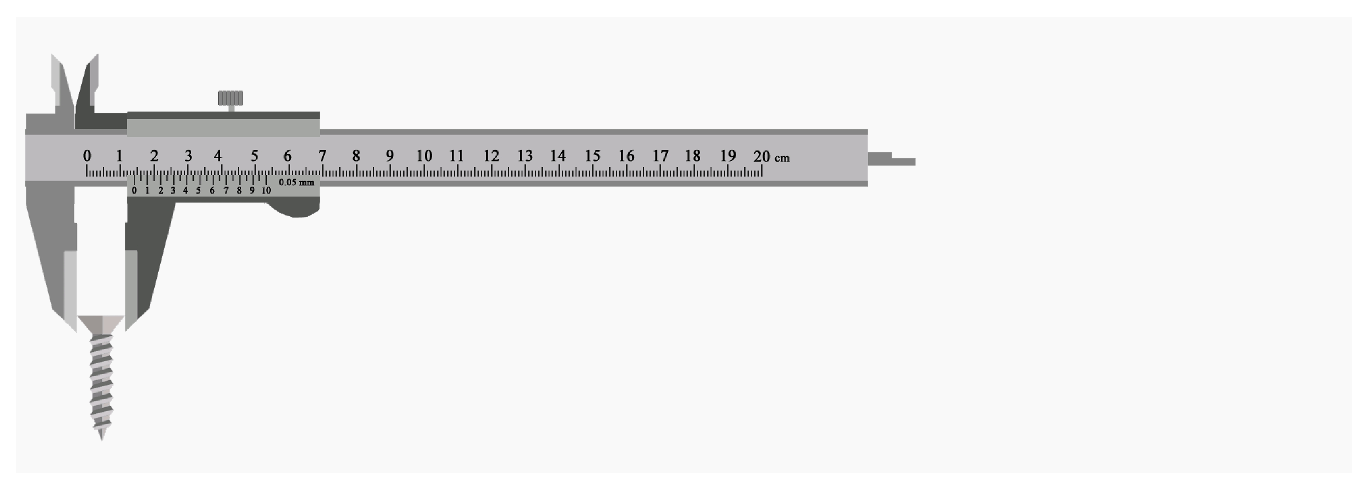
\includegraphics[width=1.0\textwidth]{resources/1_5.1.7.eps}
\end{figure}
\vspace*{0.4cm}
\scriptsize
\begin{tabular}{|c|>{\centering}m{1.8cm}<{\centering}|}
\hline
$X_{rep}$ &  $14.10$ \tabularnewline \hline
      $P$ &   $0.05$ \tabularnewline \hline
      $u$ &     $mm$ \tabularnewline \hline
$E_x(\%)$ &   $0.36$ \tabularnewline \hline
\end{tabular}
\quad
\begin{tabular}{|c|>{\centering}m{5.7cm}<{\centering}|}
\hline
\multicolumn{2}{|c|}{\textbf{Resultado de la medición}} \\ \hline
$D$ & $( 14.10\pm0.05)[mm], 0.36\%$ \tabularnewline \hline
\end{tabular}
\end{frame}

\subsection{Diámetro del cuerpo del tornillo}
\begin{frame}
\frametitle{Diámetro del cuerpo del tornillo}
\vspace*{0.8cm}
\begin{figure}
\centering
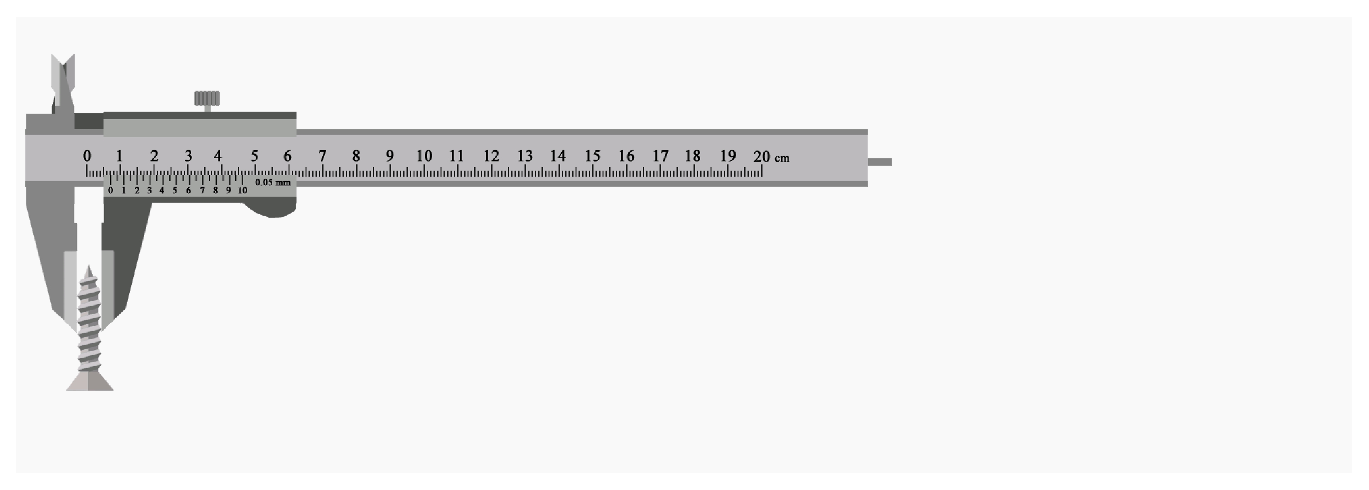
\includegraphics[width=1.0\textwidth]{resources/1_5.1.8.eps}
\end{figure}
\vspace*{0.4cm}
\scriptsize
\begin{tabular}{|c|>{\centering}m{1.8cm}<{\centering}|}
\hline
$X_{rep}$ &   $7.10$ \tabularnewline \hline
      $P$ &   $0.05$ \tabularnewline \hline
      $u$ &     $mm$ \tabularnewline \hline
$E_x(\%)$ &   $0.70$ \tabularnewline \hline
\end{tabular}
\quad
\begin{tabular}{|c|>{\centering}m{5.7cm}<{\centering}|}
\hline
\multicolumn{2}{|c|}{\textbf{Resultado de la medición}} \\ \hline
$D$ & $(  7.10\pm0.05)[mm], 0.70\%$ \tabularnewline \hline
\end{tabular}
\end{frame}

\subsection{Longitud de la cabeza del tornillo}
\begin{frame}
\frametitle{Longitud de la cabeza del tornillo}
\vspace*{0.8cm}
\begin{figure}
\centering
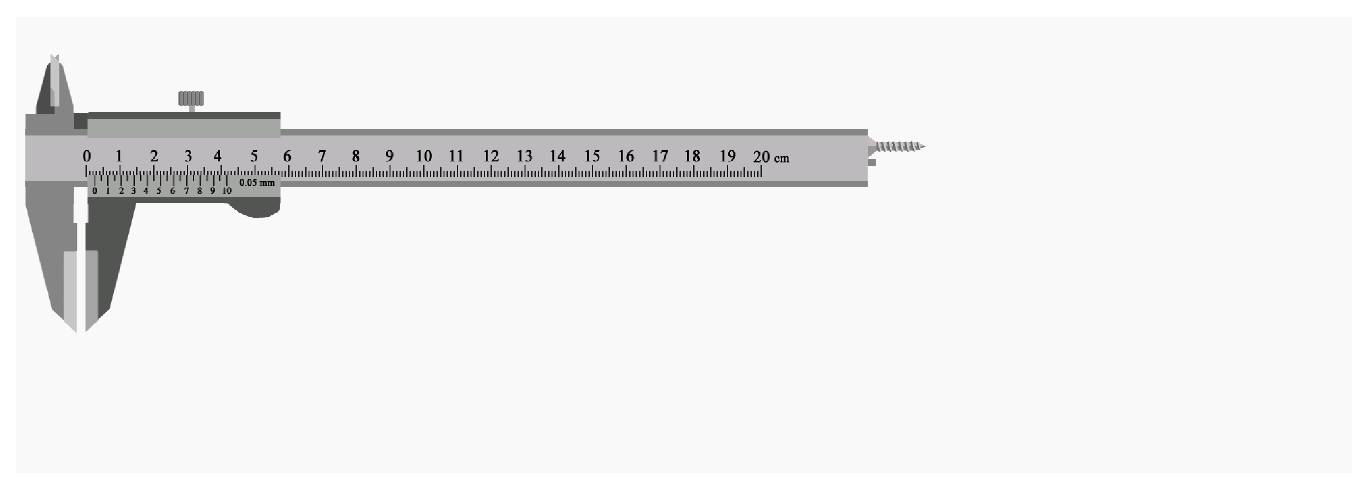
\includegraphics[width=1.0\textwidth]{resources/1_5.1.9.eps}
\end{figure}
\vspace*{0.4cm}
\scriptsize
\begin{tabular}{|c|>{\centering}m{1.8cm}<{\centering}|}
\hline
$X_{rep}$ &   $2.55$ \tabularnewline \hline
      $P$ &   $0.05$ \tabularnewline \hline
      $u$ &     $mm$ \tabularnewline \hline
$E_x(\%)$ &   $1.96$ \tabularnewline \hline
\end{tabular}
\quad
\begin{tabular}{|c|>{\centering}m{5.7cm}<{\centering}|}
\hline
\multicolumn{2}{|c|}{\textbf{Resultado de la medición}} \\ \hline
$L$ & $( 2.55\pm0.05)[mm], 1.96\%$ \tabularnewline \hline
\end{tabular}
\end{frame}

\subsection{Longitud del cuerpo del tornillo}
\begin{frame}
\frametitle{Longitud del cuerpo del tornillo}
\vspace*{0.8cm}
\begin{figure}
\centering
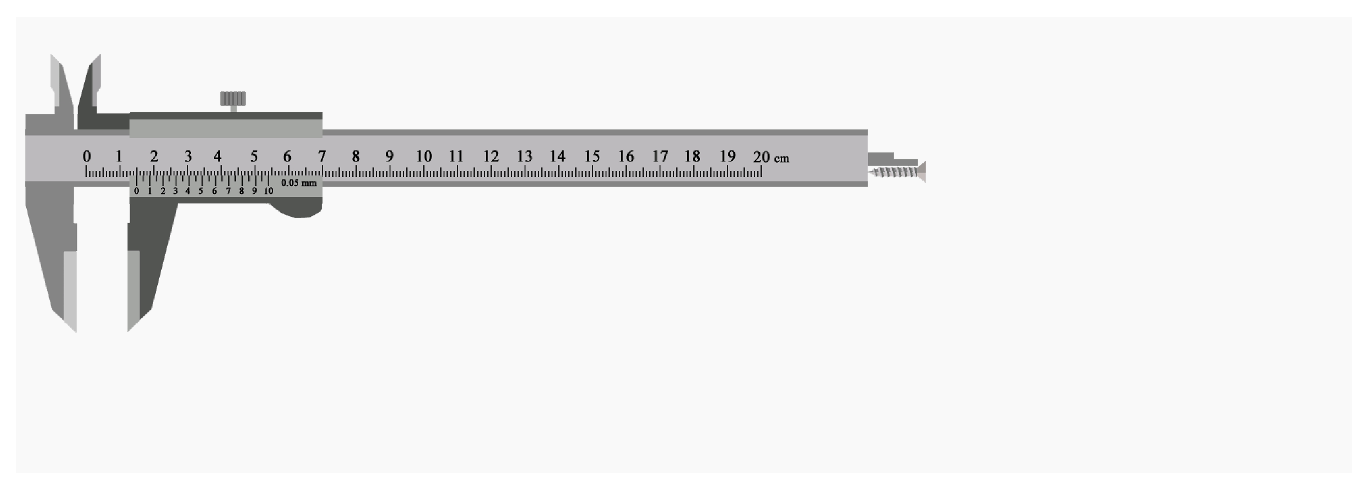
\includegraphics[width=1.0\textwidth]{resources/1_5.1.10.eps}
\end{figure}
\vspace*{0.4cm}
\scriptsize
\begin{tabular}{|c|>{\centering}m{1.8cm}<{\centering}|}
\hline
$X_{rep}$ &  $15.00$ \tabularnewline \hline
      $P$ &   $0.05$ \tabularnewline \hline
      $u$ &     $mm$ \tabularnewline \hline
$E_x(\%)$ &   $0.34$ \tabularnewline \hline
\end{tabular}
\quad
\begin{tabular}{|c|>{\centering}m{5.7cm}<{\centering}|}
\hline
\multicolumn{2}{|c|}{\textbf{Resultado de la medición}} \\ \hline
$L$ & $( 15.00\pm0.05)[mm], 0.34\%$ \tabularnewline \hline
\end{tabular}
\end{frame}

\subsection{Longitud total del tornillo}
\begin{frame}
\frametitle{Longitud total del tornillo}
\vspace*{0.8cm}
\begin{figure}
\centering
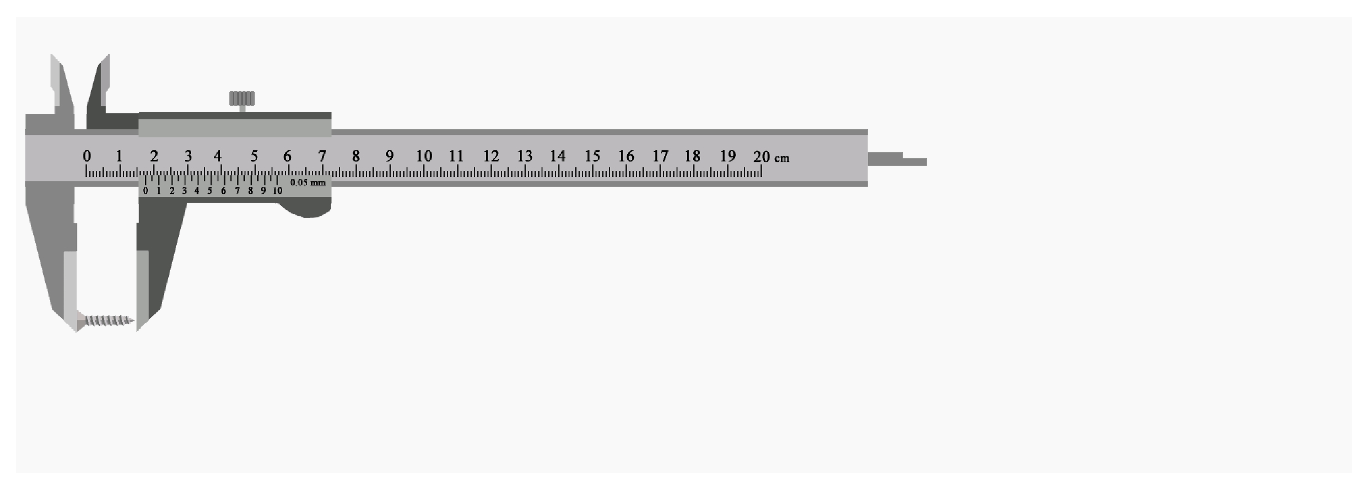
\includegraphics[width=1.0\textwidth]{resources/1_5.1.11.eps}
\end{figure}
\vspace*{0.4cm}
\scriptsize
\begin{tabular}{|c|>{\centering}m{1.8cm}<{\centering}|}
\hline
$X_{rep}$ &  $17.55$ \tabularnewline \hline
      $P$ &   $0.05$ \tabularnewline \hline
      $u$ &     $mm$ \tabularnewline \hline
$E_x(\%)$ &   $0.28$ \tabularnewline \hline
\end{tabular}
\quad
\begin{tabular}{|c|>{\centering}m{5.7cm}<{\centering}|}
\hline
\multicolumn{2}{|c|}{\textbf{Resultado de la medición}} \\ \hline
$L$ & $( 17.55\pm0.05)[mm], 0.28\%$ \tabularnewline \hline
\end{tabular}
\end{frame}

\subsection{Longitud externa de la pieza}
\begin{frame}
\frametitle{Longitud externa de la pieza}
\vspace*{0.8cm}
\begin{figure}
\centering
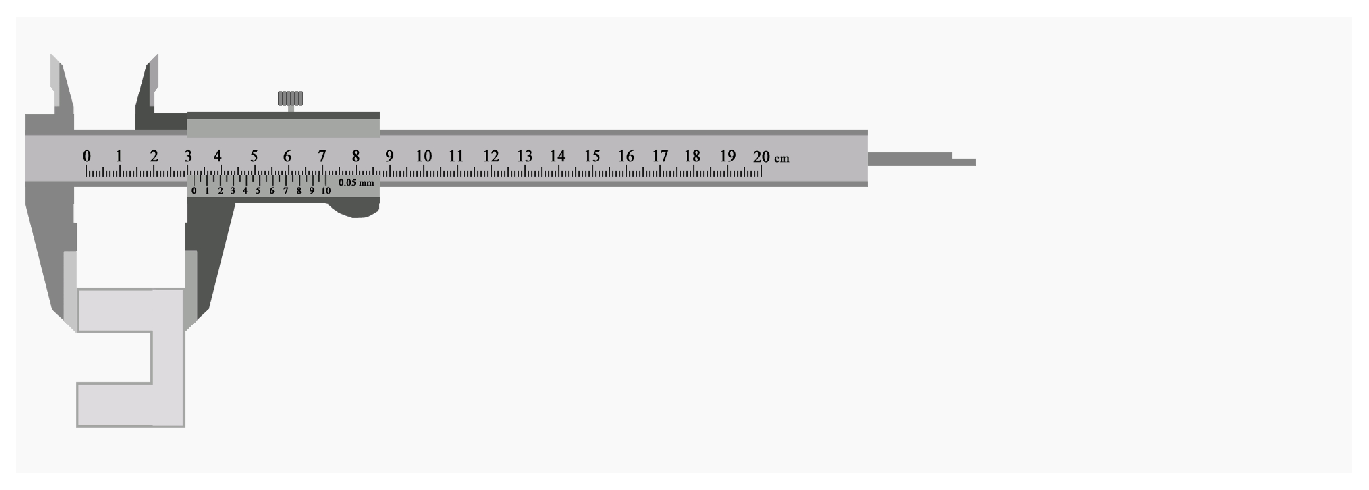
\includegraphics[width=1.0\textwidth]{resources/1_5.1.12.eps}
\end{figure}
\vspace*{0.4cm}
\scriptsize
\begin{tabular}{|c|>{\centering}m{1.8cm}<{\centering}|}
\hline
$X_{rep}$ &  $32.00$ \tabularnewline \hline
      $P$ &   $0.05$ \tabularnewline \hline
      $u$ &     $mm$ \tabularnewline \hline
$E_x(\%)$ &   $0.16$ \tabularnewline \hline
\end{tabular}
\quad
\begin{tabular}{|c|>{\centering}m{5.7cm}<{\centering}|}
\hline
\multicolumn{2}{|c|}{\textbf{Resultado de la medición}} \\ \hline
$L$ & $( 32.00\pm0.05)[mm], 0.16\%$ \tabularnewline \hline
\end{tabular}
\end{frame}

\subsection{Longitud interna de la pieza}
\begin{frame}
\frametitle{Longitud interna de la pieza}
\vspace*{0.8cm}
\begin{figure}
\centering
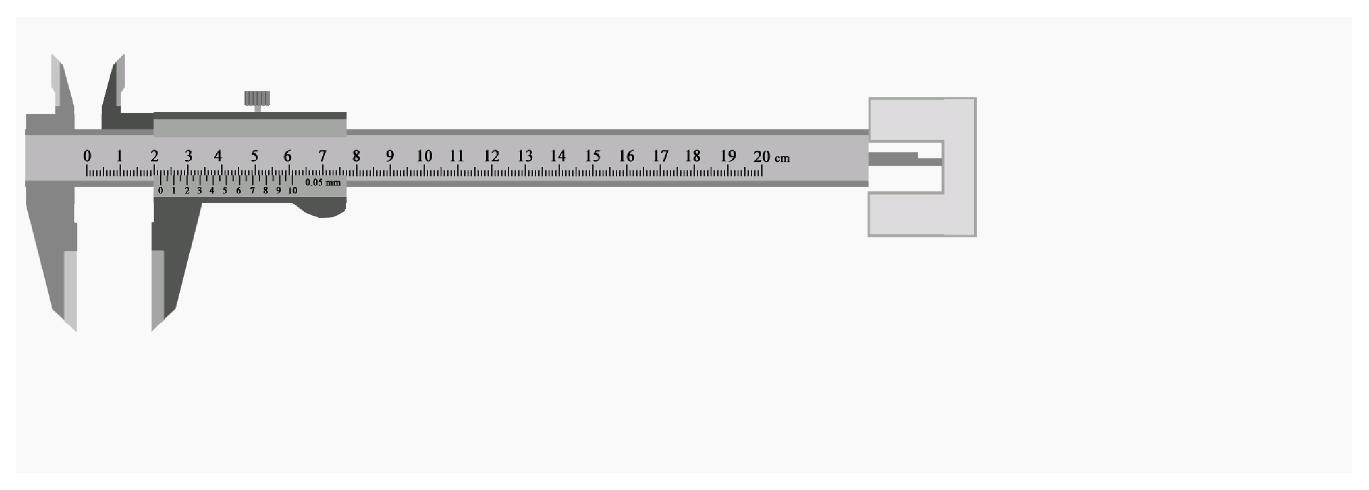
\includegraphics[width=1.0\textwidth]{resources/1_5.1.13.eps}
\end{figure}
\vspace*{0.4cm}
\scriptsize
\begin{tabular}{|c|>{\centering}m{1.8cm}<{\centering}|}
\hline
$X_{rep}$ &  $22.00$ \tabularnewline \hline
      $P$ &   $0.05$ \tabularnewline \hline
      $u$ &     $mm$ \tabularnewline \hline
$E_x(\%)$ &   $0.23$ \tabularnewline \hline
\end{tabular}
\quad
\begin{tabular}{|c|>{\centering}m{5.7cm}<{\centering}|}
\hline
\multicolumn{2}{|c|}{\textbf{Resultado de la medición}} \\ \hline
$L$ & $( 22.00\pm0.05)[mm], 0.23\%$ \tabularnewline \hline
\end{tabular}
\end{frame}

\subsection{Longitud externa de la pieza}
\begin{frame}
\frametitle{Longitud externa de la pieza}
\vspace*{0.8cm}
\begin{figure}
\centering
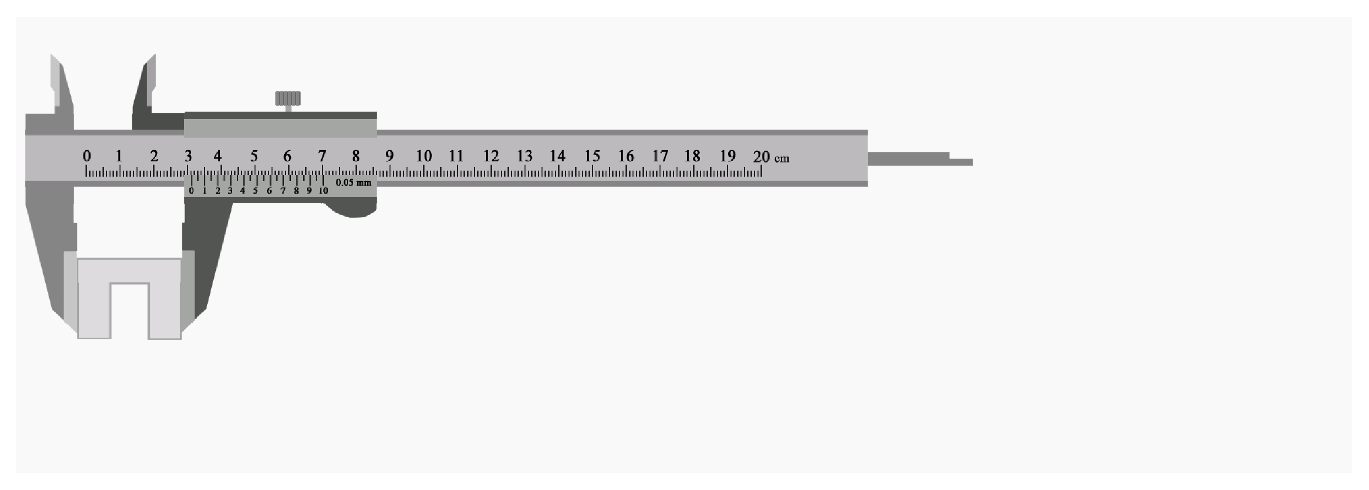
\includegraphics[width=1.0\textwidth]{resources/1_5.1.14.eps}
\end{figure}
\vspace*{0.4cm}
\scriptsize
\begin{tabular}{|c|>{\centering}m{1.8cm}<{\centering}|}
\hline
$X_{rep}$ &  $31.10$ \tabularnewline \hline
      $P$ &   $0.05$ \tabularnewline \hline
      $u$ &     $mm$ \tabularnewline \hline
$E_x(\%)$ &   $0.16$ \tabularnewline \hline
\end{tabular}
\quad
\begin{tabular}{|c|>{\centering}m{5.7cm}<{\centering}|}
\hline
\multicolumn{2}{|c|}{\textbf{Resultado de la medición}} \\ \hline
$L$ & $( 31.10\pm0.05)[mm], 0.16\%$ \tabularnewline \hline
\end{tabular}
\end{frame}

\subsection{Longitud interna de la pieza}
\begin{frame}
\frametitle{Longitud interna de la pieza}
\vspace*{0.8cm}
\begin{figure}
\centering
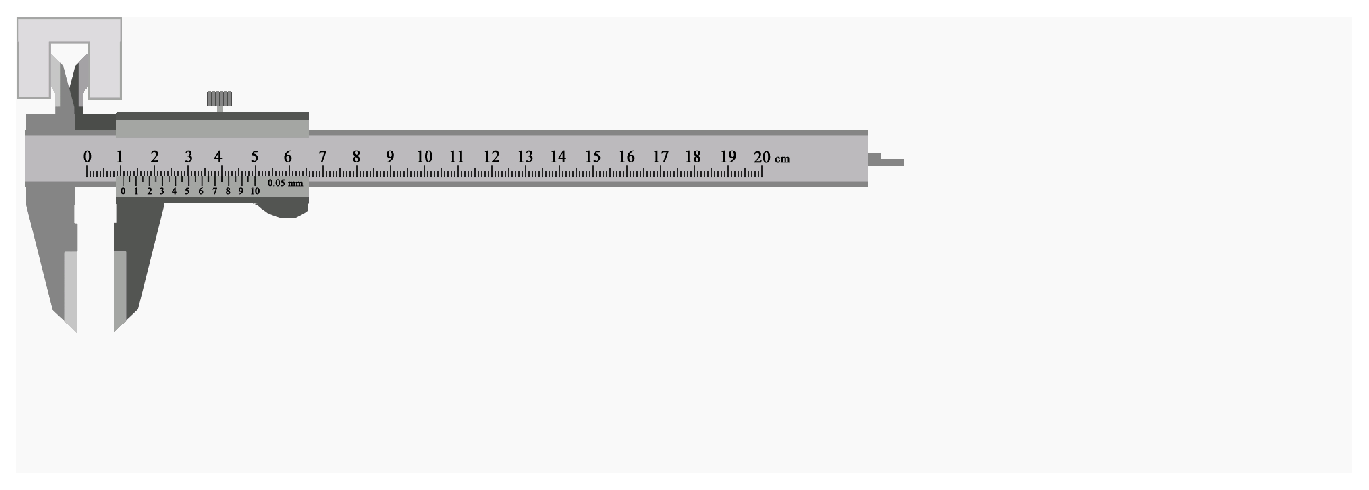
\includegraphics[width=1.0\textwidth]{resources/1_5.1.15.eps}
\end{figure}
\vspace*{0.4cm}
\scriptsize
\begin{tabular}{|c|>{\centering}m{1.8cm}<{\centering}|}
\hline
$X_{rep}$ &  $10.70$ \tabularnewline \hline
      $P$ &   $0.05$ \tabularnewline \hline
      $u$ &     $mm$ \tabularnewline \hline
$E_x(\%)$ &   $0.47$ \tabularnewline \hline
\end{tabular}
\quad
\begin{tabular}{|c|>{\centering}m{5.7cm}<{\centering}|}
\hline
\multicolumn{2}{|c|}{\textbf{Resultado de la medición}} \\ \hline
$L$ & $( 10.70\pm0.05)[mm], 0.47\%$ \tabularnewline \hline
\end{tabular}
\end{frame}

\subsection{Longitud de la caja}
\begin{frame}
\frametitle{Longitud de la caja}
\vspace*{0.8cm}
\begin{figure}
\centering
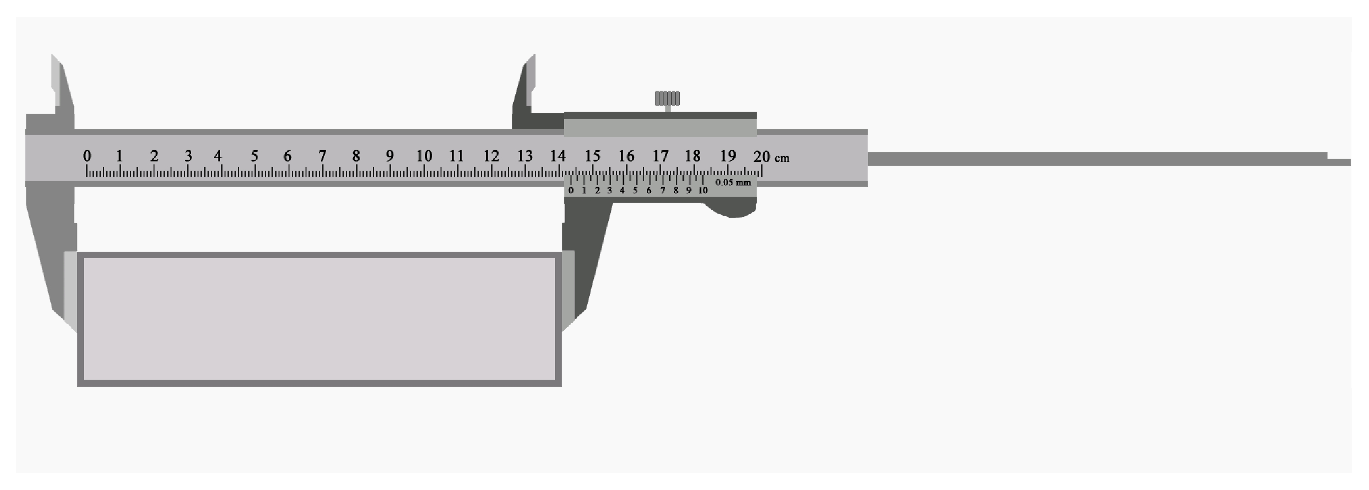
\includegraphics[width=1.0\textwidth]{resources/1_5.1.16.eps}
\end{figure}
\vspace*{0.4cm}
\scriptsize
\begin{tabular}{|c|>{\centering}m{1.8cm}<{\centering}|}
\hline
$X_{rep}$ & $143.55$ \tabularnewline \hline
      $P$ &   $0.05$ \tabularnewline \hline
      $u$ &     $mm$ \tabularnewline \hline
$E_x(\%)$ &   $0.03$ \tabularnewline \hline
\end{tabular}
\quad
\begin{tabular}{|c|>{\centering}m{5.7cm}<{\centering}|}
\hline
\multicolumn{2}{|c|}{\textbf{Resultado de la medición}} \\ \hline
$D$ & $(143.55\pm0.05)[mm], 0.03\%$ \tabularnewline \hline
\end{tabular}
\end{frame}

\section{Tornillo Micrométrico}

\subsection{Diámetro del capacitor}
\begin{frame}
\frametitle{Diámetro del capacitor}
\vspace*{0.8cm}
\begin{figure}
\centering
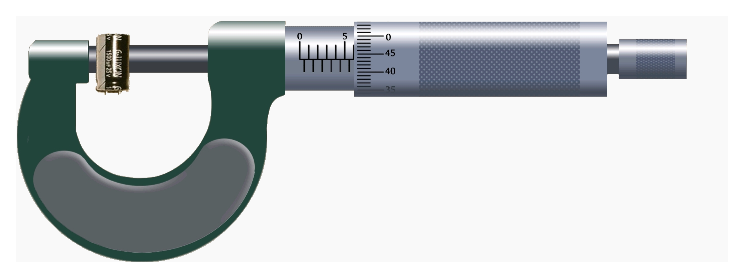
\includegraphics[width=1.0\textwidth]{resources/1_5.2.1.eps}
\end{figure}
\vspace*{0.4cm}
\scriptsize
\begin{tabular}{|c|>{\centering}m{1.8cm}<{\centering}|}
\hline
$X_{rep}$ &  $5.5+0.43$ \tabularnewline \hline
      $P$ &      $0.01$ \tabularnewline \hline
      $u$ &        $mm$ \tabularnewline \hline
$E_x(\%)$ &      $0.17$ \tabularnewline \hline
\end{tabular}
\quad
\begin{tabular}{|c|>{\centering}m{5.7cm}<{\centering}|}
\hline
\multicolumn{2}{|c|}{\textbf{Resultado de la medición}} \\ \hline
$D$ & $( 5.93\pm0.01)[mm], 0.17\%$ \tabularnewline \hline
\end{tabular}
\end{frame}

\subsection{Diámetro de la cabeza del perno}
\begin{frame}
\frametitle{Diámetro de la cabeza del perno}
\vspace*{0.8cm}
\begin{figure}
\centering
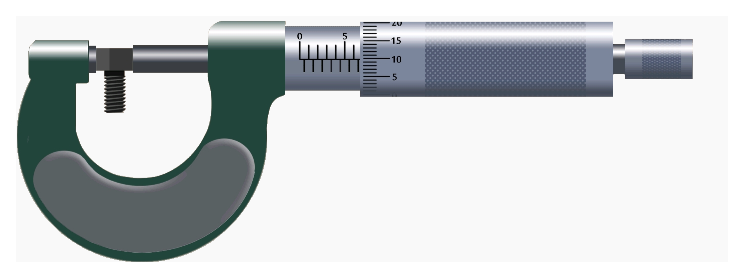
\includegraphics[width=1.0\textwidth]{resources/1_5.2.2.eps}
\end{figure}
\vspace*{0.4cm}
\scriptsize
\begin{tabular}{|c|>{\centering}m{1.8cm}<{\centering}|}
\hline
$X_{rep}$ &  $6.5+0.09$ \tabularnewline \hline
      $P$ &      $0.01$ \tabularnewline \hline
      $u$ &        $mm$ \tabularnewline \hline
$E_x(\%)$ &      $0.15$ \tabularnewline \hline
\end{tabular}
\quad
\begin{tabular}{|c|>{\centering}m{5.7cm}<{\centering}|}
\hline
\multicolumn{2}{|c|}{\textbf{Resultado de la medición}} \\ \hline
$D$ & $( 6.59\pm0.01)[mm], 0.15\%$ \tabularnewline \hline
\end{tabular}
\end{frame}

\subsection{Diámetro del cuerpo del perno}
\begin{frame}
\frametitle{Diámetro del cuerpo del perno}
\vspace*{0.8cm}
\begin{figure}
\centering
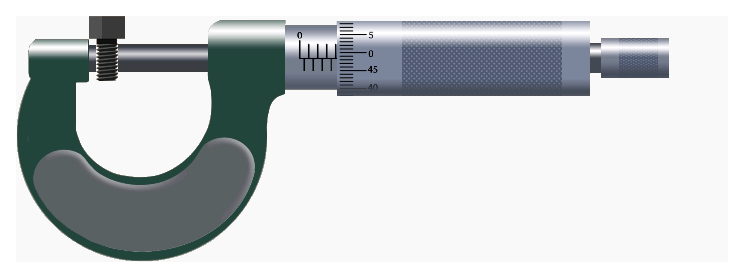
\includegraphics[width=1.0\textwidth]{resources/1_5.2.3.eps}
\end{figure}
\vspace*{0.4cm}
\scriptsize
\begin{tabular}{|c|>{\centering}m{1.8cm}<{\centering}|}
\hline
$X_{rep}$ &  $3.5+0.48$ \tabularnewline \hline
      $P$ &      $0.01$ \tabularnewline \hline
      $u$ &        $mm$ \tabularnewline \hline
$E_x(\%)$ &      $0.25$ \tabularnewline \hline
\end{tabular}
\quad
\begin{tabular}{|c|>{\centering}m{5.7cm}<{\centering}|}
\hline
\multicolumn{2}{|c|}{\textbf{Resultado de la medición}} \\ \hline
$D$ & $( 3.98\pm0.01)[mm], 0.25\%$ \tabularnewline \hline
\end{tabular}
\end{frame}

\subsection{Diámetro de la cabeza del tornillo}
\begin{frame}
\frametitle{Diámetro de la cabeza del tornillo}
\vspace*{0.8cm}
\begin{figure}
\centering
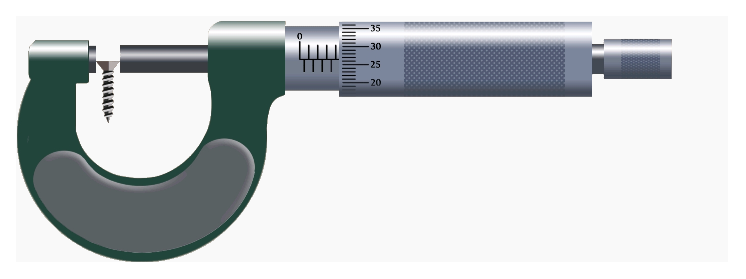
\includegraphics[width=1.0\textwidth]{resources/1_5.2.4.eps}
\end{figure}
\vspace*{0.4cm}
\scriptsize
\begin{tabular}{|c|>{\centering}m{1.8cm}<{\centering}|}
\hline
$X_{rep}$ &  $4.0+0.26$ \tabularnewline \hline
      $P$ &      $0.01$ \tabularnewline \hline
      $u$ &        $mm$ \tabularnewline \hline
$E_x(\%)$ &      $0.23$ \tabularnewline \hline
\end{tabular}
\quad
\begin{tabular}{|c|>{\centering}m{5.7cm}<{\centering}|}
\hline
\multicolumn{2}{|c|}{\textbf{Resultado de la medición}} \\ \hline
$D$ & $( 4.26\pm0.01)[mm], 0.23\%$ \tabularnewline \hline
\end{tabular}
\end{frame}

\subsection{Diámetro del cuerpo del tornillo}
\begin{frame}
\frametitle{Diámetro del cuerpo del tornillo}
\vspace*{0.8cm}
\begin{figure}
\centering
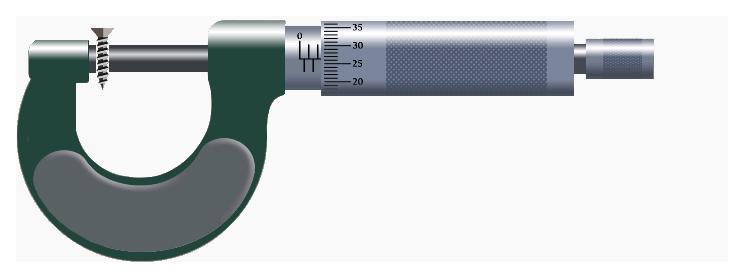
\includegraphics[width=1.0\textwidth]{resources/1_5.2.5.eps}
\end{figure}
\vspace*{0.4cm}
\scriptsize
\begin{tabular}{|c|>{\centering}m{1.8cm}<{\centering}|}
\hline
$X_{rep}$ &  $2.0+0.26$ \tabularnewline \hline
      $P$ &      $0.01$ \tabularnewline \hline
      $u$ &        $mm$ \tabularnewline \hline
$E_x(\%)$ &      $0.44$ \tabularnewline \hline
\end{tabular}
\quad
\begin{tabular}{|c|>{\centering}m{5.7cm}<{\centering}|}
\hline
\multicolumn{2}{|c|}{\textbf{Resultado de la medición}} \\ \hline
$D$ & $( 2.26\pm0.01)[mm], 0.44\%$ \tabularnewline \hline
\end{tabular}
\end{frame}

\subsection{Longitud de la cabeza del tornillo (Estimado)}
\begin{frame}
\frametitle{Longitud de la cabeza del tornillo (Estimado)}
\vspace*{0.8cm}
\begin{figure}
\centering
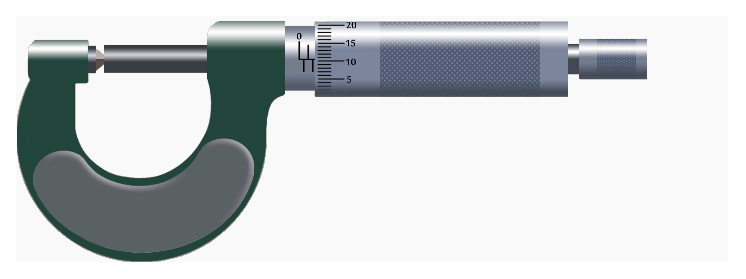
\includegraphics[width=1.0\textwidth]{resources/1_5.2.6.eps}
\end{figure}
\vspace*{0.4cm}
\scriptsize
\begin{tabular}{|c|>{\centering}m{1.8cm}<{\centering}|}
\hline
$X_{rep}$ &  $1.5+0.10$ \tabularnewline \hline
      $P$ &      $0.01$ \tabularnewline \hline
      $u$ &        $mm$ \tabularnewline \hline
$E_x(\%)$ &      $0.62$ \tabularnewline \hline
\end{tabular}
\quad
\begin{tabular}{|c|>{\centering}m{5.7cm}<{\centering}|}
\hline
\multicolumn{2}{|c|}{\textbf{Resultado de la medición}} \\ \hline
$L$ & $( 1.60\pm0.01)[mm], 0.62\%$ \tabularnewline \hline
\end{tabular}
\end{frame}

\subsection{Longitud del cuerpo del tornillo (Estimado)}
\begin{frame}
\frametitle{Longitud del cuerpo del tornillo (Estimado)}
\vspace*{0.8cm}
\begin{figure}
\centering
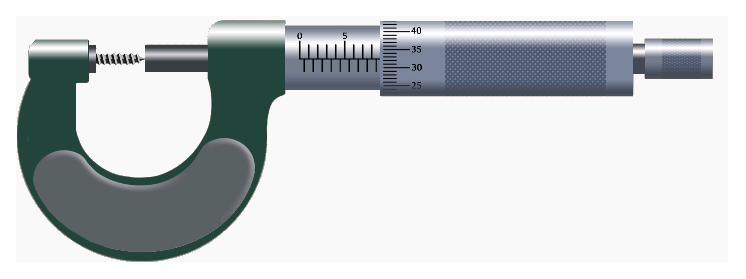
\includegraphics[width=1.0\textwidth]{resources/1_5.2.7.eps}
\end{figure}
\vspace*{0.4cm}
\scriptsize
\begin{tabular}{|c|>{\centering}m{1.8cm}<{\centering}|}
\hline
$X_{rep}$ &  $8.5+0.32$ \tabularnewline \hline
      $P$ &      $0.01$ \tabularnewline \hline
      $u$ &        $mm$ \tabularnewline \hline
$E_x(\%)$ &      $0.11$ \tabularnewline \hline
\end{tabular}
\quad
\begin{tabular}{|c|>{\centering}m{5.7cm}<{\centering}|}
\hline
\multicolumn{2}{|c|}{\textbf{Resultado de la medición}} \\ \hline
$L$ & $( 8.82\pm0.01)[mm], 0.11\%$ \tabularnewline \hline
\end{tabular}
\end{frame}

\subsection{Longitud total del tornillo}
\begin{frame}
\frametitle{Longitud total del tornillo}
\vspace*{0.8cm}
\begin{figure}
\centering
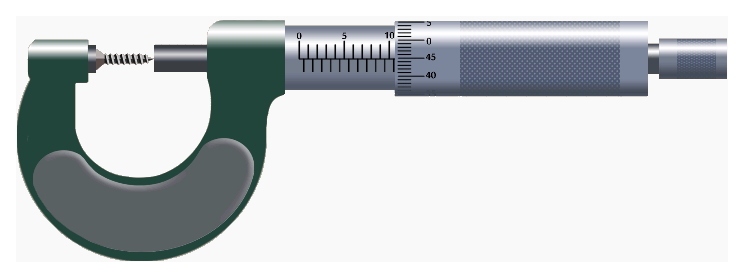
\includegraphics[width=1.0\textwidth]{resources/1_5.2.8.eps}
\end{figure}
\vspace*{0.4cm}
\scriptsize
\begin{tabular}{|c|>{\centering}m{1.8cm}<{\centering}|}
\hline
$X_{rep}$ &  $10.0+0.44$ \tabularnewline \hline
      $P$ &       $0.01$ \tabularnewline \hline
      $u$ &         $mm$ \tabularnewline \hline
$E_x(\%)$ &       $0.10$ \tabularnewline \hline
\end{tabular}
\quad
\begin{tabular}{|c|>{\centering}m{5.7cm}<{\centering}|}
\hline
\multicolumn{2}{|c|}{\textbf{Resultado de la medición}} \\ \hline
$L$ & $(10.44\pm0.01)[mm], 0.10\%$ \tabularnewline \hline
\end{tabular}
\end{frame}

\subsection{Diámetro de la esfera}
\begin{frame}
\frametitle{Diámetro de la esfera}
\vspace*{0.8cm}
\begin{figure}
\centering
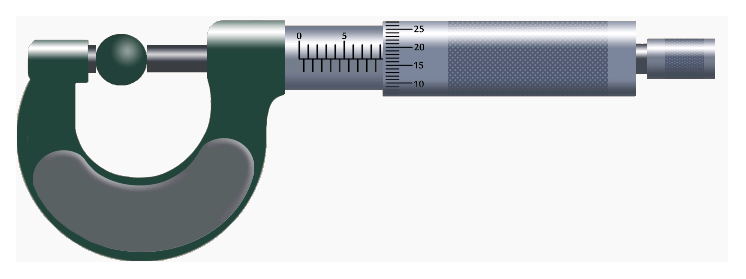
\includegraphics[width=1.0\textwidth]{resources/1_5.2.9.eps}
\end{figure}
\vspace*{0.4cm}
\scriptsize
\begin{tabular}{|c|>{\centering}m{1.8cm}<{\centering}|}
\hline
$X_{rep}$ &  $9.0+0.16$ \tabularnewline \hline
      $P$ &      $0.01$ \tabularnewline \hline
      $u$ &        $mm$ \tabularnewline \hline
$E_x(\%)$ &      $0.11$ \tabularnewline \hline
\end{tabular}
\quad
\begin{tabular}{|c|>{\centering}m{5.7cm}<{\centering}|}
\hline
\multicolumn{2}{|c|}{\textbf{Resultado de la medición}} \\ \hline
$D$ & $( 9.16\pm0.01)[mm], 0.11\%$ \tabularnewline \hline
\end{tabular}
\end{frame}

\end{document}

